\section{Math}
There are a few tricks to fixing the figures in your report, here we will show some of them.

\begin{figure}[H]
    \centering
    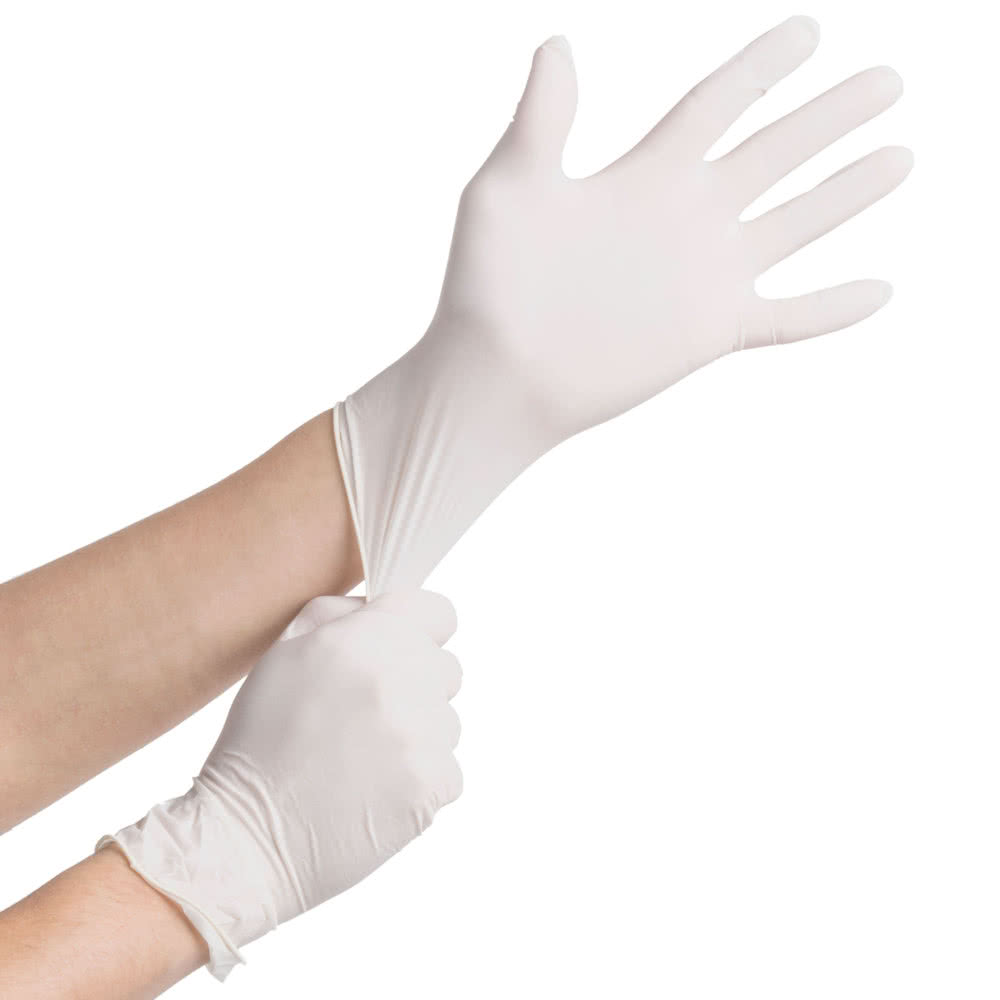
\includegraphics[scale= 0.3]{Images/Gloves.jpg}
    \caption{Vi gör oss redo för att använda Latex/Overleaf}
    \label{fig:latex}
\end{figure}


\begin{figure}[H]
    \centering
    
\includegraphics{Images/Approved.jpg}
    \caption{Damn, we got approved \citep{einstein}}
    \label{fig:chuckychuck}
\end{figure}


\begin{figure*}[t!]
    \centering
    \begin{subfigure}[t]{0.5\textwidth}
        \centering
        
\includegraphics[height=2.0in]{Images/Approved.jpg}
        \caption{Lorem ipsum}
    \end{subfigure}%
    ~ 
    \begin{subfigure}[t]{0.5\textwidth}
        \centering
        
\includegraphics[height=1.5in]{Images/Approved.jpg}
        \caption{Lorem ipsum, lorem ipsum,Lorem ipsum, lorem ipsum,Lorem ipsum}
    \end{subfigure}
    \caption{Caption place holder}
\end{figure*}


\begin{wrapfigure}{r}{0.5\textwidth}
  \begin{center}
    
\includegraphics[width=0.48\textwidth]{Images/Approved.jpg}
  \end{center}
  %\caption{HEJSAN HOPPSAN}
\end{wrapfigure}
\subsection{First Subsection in ``Second Section''}

\subsection{Second Subsection in ``Second Section''}

\subsubsection{First Subssubsection}

\subsubsection{Second Subsubsection}

\paragraph{First Paragraph}

\paragraph{Second Paragraph}


\section*{Section without numbering}

\subsection*{Subsection without numbering}

\subsubsection*{Subsubsection without numbering}
\begin{table}[H]
    \centering  
    \begin{tabular}{||c|r|l||}
        \hline 
        \textbf{Measurement using} & \textbf{Value} & \textbf{Error}\\ 
        \hline 
        SNZ  & 230 V & $\pm10^{-9000}$ V \\
        \hline
        Fluke & 215.6 V & $\pm20$ V \\
        \hline 
        Agilent & 232.1 V  & $\pm1.2$ V \\
        \hline 
        HPn & 231.3 V& $\pm0.01$ V \\
        \hline
        Z2 & 0 V & $>9000$ V \\
        \hline
        \end{tabular}
    \caption{Table from a report from Forkman}
    \label{Forkman_Mätning}
\end{table}


You don't gave to make tables such as this one from Forkman (\ref{Forkman_Mätning}), you can also make lists

\begin{enumerate}
    \item Dot 1
    \begin{enumerate}
        \item Dot 1a
        \item Dot 1b
    \end{enumerate}
\end{enumerate}

Or like this

\begin{itemize}
    \item Thing 1
    \item Thing 2
    \begin{itemize}
        \item Pinecone
        \item Pineapple
        \begin{itemize}
            \item I like Pines and SNZ
        \end{itemize}
    \end{itemize}
    \item Thing 3
    \item Thing 4
\end{itemize}

Or...

\begin{description}
    \item[Thing 1] Something 1a
    \item[Thing 2] Something 2a
\end{description}

Or like this

\begin{table}[H]
    \centering
    \begin{tabular}{r|c|l}
        Hi & ! & :D \\
        \hline
        THIS & IS & Tabular, not sparta \\
    \end{tabular}
    \caption{Box of things}
    \label{Mina_lådor_av_streck}
\end{table}


There exist a large library to make mathematical expressions in \LaTeX{}, where we will only go through a portion of them for you to familiarise your self with how it works.

\subsection{Symbols}

Many different symbols are available to use in \LaTeX{}, for example some common are:

\begin{equation}
    \textit{Just some mathimatical symbols}
\end{equation}
\begin{equation}
    \alpha, \beta, \gamma, \Gamma, \delta, \Delta, \varepsilon, \epsilon, \zeta, \eta, \Theta, \theta, \vartheta, \iota, \kappa, \varkappa, \Lambda, \lambda, \mu, \nu, \Xi
\end{equation}
\begin{equation}
    \xi, \Pi, \pi, \varpi, \rho, \varrho, \Sigma, \sigma, \varsigma, \tau, \Upsilon, \upsilon, \Phi, \phi, \varphi, \chi, \Psi, \psi, \Omega, \omega
\end{equation}

\subsection{Equations}

There are three main ways to write equations in latex, the first one is by writing one or two \$\$ signs between the equations:

$1+1=2$

$$
1-1=0
$$

You can also use the equation command in the command begin:

\begin{equation}\label{5_typ}
    2+3=5
\end{equation}

\eqref{5_typ} 
and without the numbering to the right

\begin{equation*}
    5-3 = 2
\end{equation*}

The last way is to use the align command, there as the name says. One can align the equations by using \{\}\& at the desired place to align each equation. (Obs every equation need to have it) Also to end an equation to be able to write an new equation bellow, one need to write $\backslash \backslash$ after the equation.

\begin{align}
    {}& \textit{Just som text...}\\
    {}& a = b + c\\
    {}& z = y + x\\
    \textit{This one is not alignend}
\end{align}

You can use all different kinds of things the math environment, bellow you can find a couple of examples, but it is best to google want you want or look at the latex wiki \href{https://en.wikibooks.org/wiki/LaTeX/Advanced_Mathematics}{LINK}


$$
\int^{\int^\int}_{\int_\int} \lim_{a \to \sum^{a}_{a}} \alpha \beta \gamma dt
$$

\begin{equation}
    SNZ_{cool}
    = \left(
    \lim_{SNZ \to 2 Cool 4 School} \int_{\beta}^\infty \sum_{\alpha = \beta}^{\gamma} \frac{10}{2} \cdot \frac{\pi}{\sqrt{\pi^2}}
    \right)^{Swag-i-skogen}
\end{equation}

\subsection{Other Math formulas}

Multiplications - Dot product or crossproduct

\begin{equation}
    A \times B
\end{equation}
\begin{equation}
    A \cdot B
\end{equation}

Fractions

\begin{equation}
    \frac{1}{2}
    = 0.5
\end{equation}

Matrices

$$
A = 
\begin{bmatrix}
    1 & 2 & 3 \\
    4 & 5 & 6 \\
    7 & 8 & 9 \\
\end{bmatrix}
, \qquad
b = 
\begin{bmatrix}
    10 \\
    11 \\
    12 \\
\end{bmatrix}
$$

Transpose

\begin{equation}
    A^\top
\end{equation}

Dynamic sizes of parenthesis

\begin{equation}
    \left(
    \frac{
    \left(
    \frac{\left(\frac{\left( a \right)}{b} \right) }{\left(\frac{c}{d} \right) }
    \right)
    }{d}
    \right)
\end{equation} 

Boxed in equations

\begin{equation}
    \boxed{
    x^2+y^2
    \neq (x + y)^2
    }
\end{equation}

And there are fun math too

\begin{align*}
    &\forall SNZ_{members} \exists (Cool_{members}  \subseteq SNZ_{members}) \in \mathbb{Z} \\
    &\land \\
    &\forall \mathbb{Z} \exists (Cool_{\mathbb{Z}}  \equiv SNZ_{members})
\end{align*}